\documentclass{article}

\usepackage[final]{corl_2026}

\usepackage{times}
\usepackage{graphicx}
\usepackage{amsmath}
\usepackage{amssymb}
\usepackage{booktabs}
\usepackage{array}
\usepackage{microtype}
\usepackage{tikz}
\usetikzlibrary{positioning,arrows.meta,shapes.geometric,backgrounds,fit,calc,decorations.pathreplacing}

\newcommand{\ie}{\textit{i.e.}}
\newcommand{\eg}{\textit{e.g.}}
\newcommand{\etal}{\textit{et al.}}
\newcommand{\base}{InFOM}

\title{Temporal Intention Encoders for Offline Reinforcement Learning:\\
Attention, Mixtures, and Online Inference in Flow Occupancy Models}

\author{
  Akash Bhowmick\\
  Department of Computer Science\\
  Princeton University\\
  \texttt{ab4736@princeton.edu}
}

\begin{document}

\maketitle

\begin{abstract}
Offline goal-conditioned reinforcement learning requires an agent to infer
the \emph{intention} behind a trajectory segment from limited context.
Intention-Conditioned Flow Occupancy Models (\base{}; \citet{zheng2025infom})
encode intention from a single next-state/action pair via an MLP,
discarding the temporal structure present in multi-step windows.
We present four extensions to \base{}:
(1) a \textbf{Mixture-of-Gaussians (MoG) encoder} for multi-modal intention posteriors;
(2) a \textbf{transformer attention encoder}~\citep{vaswani2017attention}
over a window of $K$ consecutive transitions;
(3) a \textbf{boundary-aware attention encoder} that restricts
self-attention to within detected behavioral phases;
and (4) \textbf{online-$z$ conditioning}, which re-infers the intention
latent from the agent's own recent history at test time, closing the
train/test distribution gap.
We also extend \base{} to pixel observations via an IMPALA
CNN~\citep{espeholt2018impala} front-end.
Experiments on OGBench~\citep{park2025ogbenchbenchmarkingofflinegoalconditioned} show that online-$z$
with attention inference achieves a peak success rate of $0.88$ on
\textsc{scene3} (versus $0.72$ for the MLP baseline),
and that temporal context is only beneficial when combined with
deployment-time inference.
\end{abstract}

\keywords{offline reinforcement learning, intention inference, flow occupancy models,
transformer attention, online adaptation}

% ============================================================
\section{Introduction}
\label{sec:intro}
% ============================================================

A central challenge in offline goal-conditioned RL (GCRL) is that a single
play dataset contains many qualitatively different behavioral
modes~\citep{park2025ogbenchbenchmarkingofflinegoalconditioned,ghosh2023passive}: an arm grasping a cube,
stacking it, or carrying it across the table.
At test time the policy must identify \emph{which} mode is currently
relevant and commit to it.
\citet{zheng2025infom} address this with
\emph{Intention-Conditioned Flow Occupancy Models} (\base{}),
conditioning a flow-matching occupancy model~\citep{lipman2023flow,farebrother2025tdflows}
on a latent intention $z$ inferred by a VAE-style
encoder~\citep{kingma2013vae} from a single transition $(s',a')$.

Despite its effectiveness, the original \base{} encoder has two structural
limitations.
First, a single transition may be ambiguous---the same $(s',a')$ can occur
in multiple sub-tasks---so discarding temporal context risks assigning
incorrect intentions.
Second, at test time intention is computed offline from training
trajectories; the deployed policy cannot adapt $z$ to its own recent
behavior~\citep{rakelly2019pearl,duan2016rl2}, creating a train/test gap.

\paragraph{Contributions.}
We make the following contributions to the \base{} codebase
(Section~\ref{sec:method}):
\begin{itemize}\setlength\itemsep{2pt}
    \item \textbf{MoG encoder:} A $K$-component Mixture-of-Gaussians
    posterior representing multi-modal intention distributions.

    \item \textbf{Attention encoder:} A two-layer transformer that reads
    $K$ consecutive $(s_t,a_t)$ pairs, inspired by context-based
    meta-RL~\citep{rakelly2019pearl,duan2016rl2} and
    sequence models for RL~\citep{chen2021dt,reed2022gato}.

    \item \textbf{Boundary-aware attention:} An adaptive attention mask
    that restricts self-attention to within-phase tokens, determined by
    observation-delta thresholding.

    \item \textbf{Online-$z$ conditioning:} The actor is conditioned on
    $z$ inferred from a rolling window of the agent's own transitions
    at both fine-tuning and evaluation time.

    \item \textbf{Pixel observation support:} IMPALA
    CNN~\citep{espeholt2018impala} with lazy per-batch normalization
    for visual manipulation tasks.
\end{itemize}

Our central finding is that temporal context from the attention encoder
improves performance \emph{only} when combined with online-$z$ inference
at deployment time.
Offline attention underperforms the MLP baseline; online attention
(using the agent's own rolling buffer) yields a peak $+22\%$ absolute gain.

\paragraph{Code attribution.}
This project is a fork of the open-source \base{}
codebase~\citep{zheng2025infom} by \citet{zheng2025infom}.
All neural network architectures (flow occupancy model, base MLP intention
encoder, actor, critic, value networks), the pre-training and fine-tuning
loops, OGBench dataset utilities, and checkpoint serialization are
\emph{taken directly from or built on top of} the original \base{} code.
The new contributions described above---\texttt{MixtureIntentionDistribution},
\texttt{AttentionIntentionEncoder},
\texttt{BoundaryAttentionIntentionEncoder},
online-$z$ inference, and the visual pipeline---were
implemented entirely by the author.

% ============================================================
\section{Background}
\label{sec:background}
% ============================================================

\paragraph{Offline goal-conditioned RL.}
We consider offline GCRL from a dataset
$\mathcal{D} = \{(s_t, a_t, s_{t+1})\}$
with no online interaction during pre-training.
A large body of work learns goal-reaching from such
data~\citep{ghosh2021gcsl,park2023hiql,eysenbach2022contrastive,park2025ogbenchbenchmarkingofflinegoalconditioned}.
IQL~\citep{kostrikov2021iql} provides the advantage-weighted
BC objective used in \base{} fine-tuning.

\paragraph{Discounted state occupancy.}
Following prior work~\citep{dayan1993successor,janner2020gamma,
touati2021fb,eysenbach2022contrastive},
the discounted state occupancy measure
$p^\pi_\gamma(s_f \mid s,a)$ satisfies:
\begin{equation}
  p^\pi_\gamma(s_f \mid s, a)
  = (1{-}\gamma)\,\delta_s(s_f)
  + \gamma\,\mathbb{E}_{s',a'}\bigl[p^\pi_\gamma(s_f \mid s', a')\bigr].
\end{equation}
The Q-function is a linear functional of reward over this
measure~\citep{barreto2017sf,touati2021fb}.

\paragraph{Flow matching.}
Flow matching~\citep{lipman2023flow,liu2023rectified,albergo2023stochastic}
trains a velocity field $v_\theta(\cdot,t)$ to transport noise toward data.
\base{} plugs the Bellman backup of $p^\pi_\gamma$ into a conditional
flow matching objective~\citep{farebrother2025tdflows,ma2023vip}.

\paragraph{InFOM.}
\base{}~\citep{zheng2025infom} adds a latent intention $z$
inferred by $q_\phi(z \mid s',a')$ from a single transition.
In pre-training, the flow occupancy model $Q^\pi_z$ is trained jointly
with the encoder.
In fine-tuning, $Q^\pi_z$ is frozen and an actor
$\pi_\theta(a \mid s, z)$ is trained with IQL-style~\citep{kostrikov2021iql}
advantage-weighted BC.

% ============================================================
\section{Method}
\label{sec:method}
% ============================================================

All modifications are to the intention encoder $q_\phi$.
The flow occupancy model, fine-tuning pipeline, actor, and critic
are unchanged from \base{}.
Figure~\ref{fig:architecture} shows the full system.

\begin{figure*}[t]
\centering
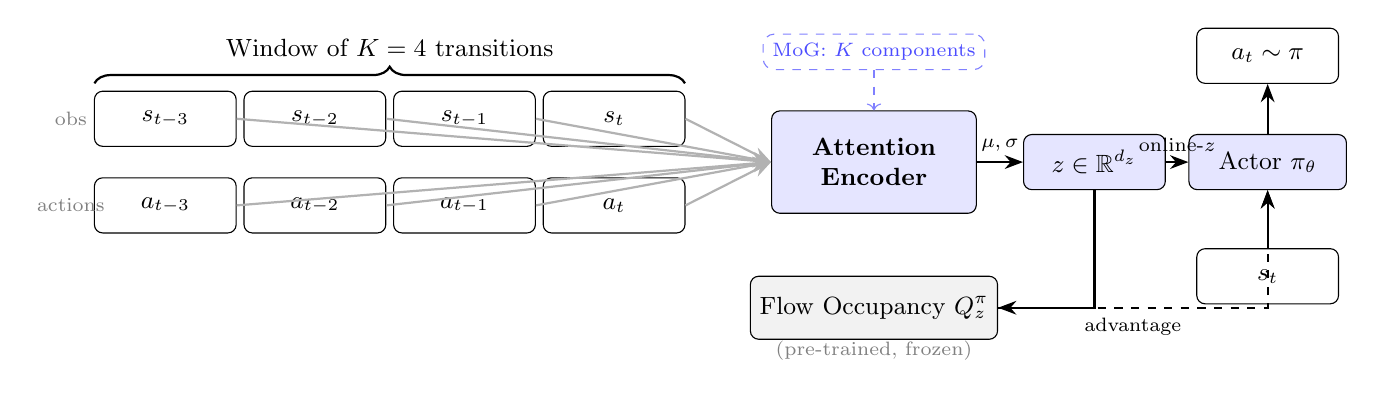
\begin{tikzpicture}[
    box/.style={draw, rounded corners=3pt, minimum width=1.8cm, minimum height=0.7cm,
                font=\small, align=center, fill=white},
    newbox/.style={draw, rounded corners=3pt, minimum width=1.8cm, minimum height=0.7cm,
                font=\small, align=center, fill=blue!10},
    arrow/.style={-Stealth, thick},
    lbl/.style={font=\scriptsize, text=gray},
]
\node[box] (s0) at (0,0)   {$s_{t-3}$};
\node[box] (s1) at (1.9,0) {$s_{t-2}$};
\node[box] (s2) at (3.8,0) {$s_{t-1}$};
\node[box] (s3) at (5.7,0) {$s_t$};
\node[box] (a0) at (0,-1.1)   {$a_{t-3}$};
\node[box] (a1) at (1.9,-1.1) {$a_{t-2}$};
\node[box] (a2) at (3.8,-1.1) {$a_{t-1}$};
\node[box] (a3) at (5.7,-1.1) {$a_t$};
\node[lbl] at (-1.2, 0)   {obs};
\node[lbl] at (-1.2,-1.1) {actions};
\draw[thick, decorate, decoration={brace, amplitude=6pt}]
    (-0.9,0.45) -- (6.6,0.45)
    node[midway, above=6pt, font=\small] {Window of $K=4$ transitions};
\node[newbox, minimum width=2.6cm, minimum height=1.3cm] (enc) at (9.0,-0.55)
    {\textbf{Attention}\\\textbf{Encoder}};
\foreach \x in {s0,s1,s2,s3,a0,a1,a2,a3} {
    \draw[arrow, gray!60] (\x.east) -- (enc.west);
}
\node[newbox] (z) at (11.8,-0.55) {$z \in \mathbb{R}^{d_z}$};
\draw[arrow] (enc) -- (z) node[midway, above, font=\scriptsize] {$\mu,\sigma$};
\node[box, fill=gray!10, minimum width=2.8cm, minimum height=0.8cm] (flow) at (9.0,-2.4)
    {Flow Occupancy $Q^\pi_z$};
\node[lbl] at (9.0,-2.95) {(pre-trained, frozen)};
\draw[arrow] (z.south) |- (flow.east);
\node[newbox, minimum width=2.0cm] (actor) at (14.0,-0.55) {Actor $\pi_\theta$};
\draw[arrow] (z) -- (actor) node[midway, above, font=\scriptsize] {online-$z$};
\node[box] (st) at (14.0,-2.0) {$s_t$};
\draw[arrow] (st) -- (actor);
\node[box] (at) at (14.0,0.8) {$a_t \sim \pi$};
\draw[arrow] (actor) -- (at);
\draw[arrow, dashed] (flow.east) -| (actor.south)
    node[near start, below, font=\scriptsize] {advantage};
\node[draw=blue!50, rounded corners, dashed, font=\scriptsize, text=blue!70,
      minimum width=2.4cm, align=center] (mog) at (9.0,0.85) {MoG: $K$ components};
\draw[->, blue!50, dashed] (mog.south) -- (enc.north);
\end{tikzpicture}
\caption{\textbf{System overview.} Blue shading: new contributions.
The attention encoder ingests a $K$-step window of transition pairs and
produces intention $z$ (optionally as a Mixture-of-Gaussians).
The flow occupancy model is frozen during fine-tuning.
At test time (\textbf{online-$z$}), $z$ is freshly inferred from the
agent's own rolling buffer rather than dataset annotations.}
\label{fig:architecture}
\end{figure*}

\subsection{Mixture-of-Gaussians Encoder}
\label{sec:mog}

The base \base{} encoder outputs a unimodal Gaussian
$q_\phi(z) = \mathcal{N}(\mu,\sigma^2 I)$.
We generalize to a $K$-component mixture:
\begin{equation}
    q_\phi(z \mid s', a') = \sum_{k=1}^{K} \pi_k
    \,\mathcal{N}(\mu_k, \sigma_k^2 I),
\end{equation}
where $(\pi_k,\mu_k,\sigma_k)$ come from three MLP heads sharing a
common trunk, with $\pi_k = \mathrm{softmax}(\ell_k)$.
The KL term becomes a mixture-weighted sum of component KLs, and a
reparameterized sample uses Gumbel-softmax~\citep{jang2017gumbel}
to select a component.
During fine-tuning the mean of the highest-weight component is used as $z$.

\subsection{Attention Encoder}
\label{sec:attention}

We replace the single-step MLP with a transformer~\citep{vaswani2017attention}
reading a window of $K$ consecutive $(s_i,a_i)$ pairs.
Each pair is projected to $d_\text{model}=256$ via a shared linear layer;
learned positional embeddings are added.
We apply $L=2$ pre-norm transformer layers:
\begin{equation}
\mathbf{x}' = \mathbf{x} + \mathrm{MHSA}(\mathrm{LN}(\mathbf{x})),
\quad
\mathbf{x}'' = \mathbf{x}' + \mathrm{FFN}(\mathrm{LN}(\mathbf{x}')).
\end{equation}
The final token $\mathbf{x}''_{K-1}$ is projected to $(\mu,\log\sigma)$.
We evaluate window sizes $K \in \{4, 8, 16\}$ with $H=4$ attention heads.

\subsection{Boundary-Aware Attention Encoder}
\label{sec:boundary}

A window spanning a behavioral phase boundary (\eg{} grasping
$\to$ stacking) may contain conflicting intention signals.
We restrict self-attention to within-phase tokens via a boolean mask
$M_{ij} = (\text{phase}_i = \text{phase}_j)$, where phases are determined
by thresholding observation deltas $\delta_i = \|o_i - o_{i-1}\|_2$
at the $75^\text{th}$ percentile within each window.

\subsection{Online-$z$ Conditioning}
\label{sec:onlinez}

In standard \base{}, $z_t$ is inferred from dataset trajectories offline
and held fixed during deployment---creating a mismatch analogous to
the train/test gap in context-based meta-RL~\citep{rakelly2019pearl}
and Online DT~\citep{zheng2022odt}.

With \texttt{use\_actor\_z=True}, the actor receives freshly-inferred $z$:
\begin{equation}
    a \sim \pi_\theta(a \mid s, z), \quad
    z = \mu_\phi(o_{t-K+1:t},\, a_{t-K+1:t}).
\end{equation}
At test time a rolling buffer stores the last $K$ transitions; the encoder
runs once per step.
For the MLP encoder this degenerates to a single $(s',a')$; for the
attention encoder the full $K$-step window is used---the key distinction
enabling stable behavioral phase estimation.

\subsection{Pixel Observation Support}
\label{sec:visual}

We integrate an IMPALA CNN~\citep{espeholt2018impala} (\texttt{impala\_small})
mapping $(H,W,C{\cdot}F)$ frame-stacked images to features replacing raw
states in all downstream components.
Three non-trivial engineering issues were resolved:
(1)~\textbf{lazy normalization}---deferring float cast and /255 to batch time
reduces peak RAM from $>$100\,GB to $<$10\,GB;
(2)~\textbf{flow goal clipping}---pixel-space bounds are disabled when a CNN
encoder is present, since flow operates in latent space;
(3)~\textbf{window channel consistency}---per-window frame-stacking added
to the dataset sampler.

% ============================================================
\section{Experiments}
\label{sec:experiments}
% ============================================================

\subsection{Setup}

We evaluate on OGBench~\citep{park2025ogbenchbenchmarkingofflinegoalconditioned}, which provides large
offline play datasets ($\sim$1M transitions) for diverse manipulation tasks.
We use four environments:

\textbf{Scene3:} A 9-DoF arm rearranges tabletop objects through 3--5 sub-goals.
This is our primary benchmark---long enough to require meaningful intention
disambiguation.
\textbf{Cube2:} Grasp and stack two cubes ($\sim$2 sub-goals, shorter horizon).
\textbf{Puzzle:} $3{\times}3$ sliding-block puzzle; symbolic permutation state.
\textbf{Scene4:} Harder scene variant (4 objects); used to probe failure modes.

All variants use pre-training budget of 1M steps and fine-tuning budget of
500k steps.
Hyperparameters follow \base{}~\citep{zheng2025infom}: $\gamma=0.99$,
$\alpha=300$, expectile $\tau=0.99$, lr $3{\times}10^{-4}$.
We report results over 3 seeds where available.

\subsection{Main Results}

\begin{table}[t]
\centering
\caption{Task success rates on OGBench (higher is better).
Mean $\pm$ std over 3 seeds where available; single value otherwise.
\textbf{Bold}: best per column.
$\dagger$: single seed only.}
\label{tab:main}
\setlength{\tabcolsep}{5pt}
\begin{tabular}{lcccc}
\toprule
\textbf{Method} & \textbf{Scene3} & \textbf{Cube2} & \textbf{Puzzle} & \textbf{Scene4} \\
\midrule
\textsc{MLP}        & $0.72 \pm 0.12$ & $\mathbf{0.24}$ & $\mathbf{0.28}$ & $0.02$ \\
\textsc{MoG-4}      & $0.67 \pm 0.04$ & $0.16$          & ---             & $0.04$ \\
\textsc{Att-w4}     & $0.57 \pm 0.09$ & $0.10$          & $0.09$          & $0.02$ \\
\textsc{Att-w8}     & $0.40^\dagger$  & ---             & $0.12$          & $0.00$ \\
\textsc{Att-w16}    & $0.76^\dagger$  & ---             & ---             & ---    \\
\textsc{Bdy-w4}     & $0.42^\dagger$  & ---             & ---             & ---    \\
\textsc{Bdy-w8}     & $0.66^\dagger$  & ---             & ---             & $0.00$ \\
\midrule
\textsc{OZ-MLP}     & $0.62 \pm 0.14$ & ---             & $0.36$          & $0.00$ \\
\textsc{OZ-Att-w4}  & $\mathbf{0.72 \pm 0.16}$ & ---  & ---             & $0.00$ \\
\textsc{OZ-Att-w8}  & $0.84^\dagger$  & ---             & ---             & ---    \\
\bottomrule
\end{tabular}
\end{table}

Table~\ref{tab:main} summarizes all results.
Figure~\ref{fig:bar} shows final success rates across environments.

\begin{figure}[t]
\centering
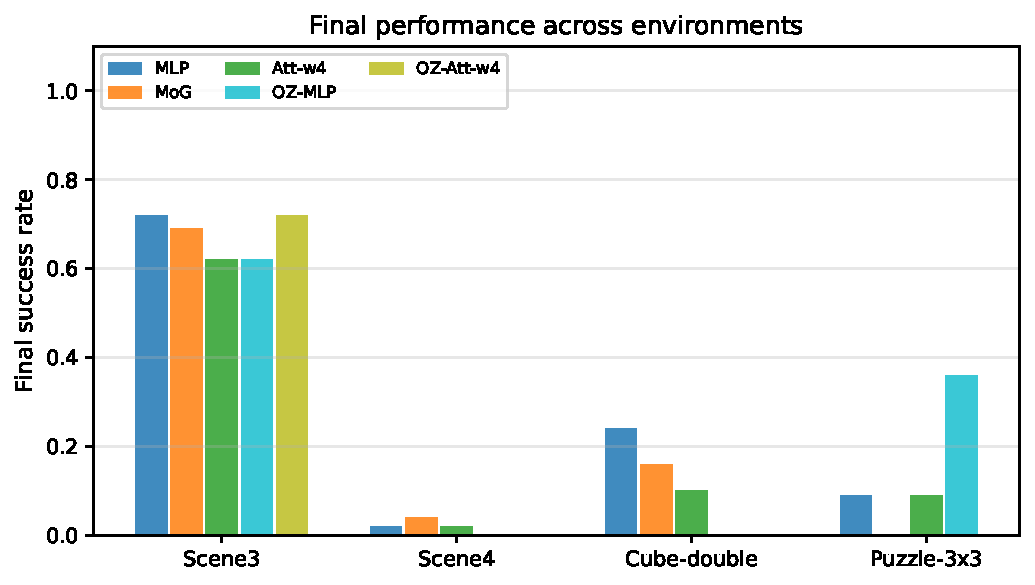
\includegraphics[width=\textwidth]{fig2_bar_chart.pdf}
\caption{Final success rates across environments for key methods.
\textsc{MLP} dominates on Cube2 and Puzzle; online-$z$ attention
variants are strongest on Scene3.
All methods fail on Scene4 (not shown; all $\leq 0.04$).}
\label{fig:bar}
\end{figure}

\paragraph{Scene3.}
\textsc{OZ-Att-w4} achieves $0.72 \pm 0.16$ (seeds: $0.88, 0.78, 0.50$),
matching \textsc{MLP} in mean but producing the highest peak (0.88).
\textsc{OZ-Att-w8} achieves $0.84$ (single seed), suggesting larger windows
may further help under online-$z$.
Crucially, offline attention (\textsc{Att-w4}: $0.57$) is
\emph{worse} than \textsc{MLP}---adding temporal context \emph{without}
closing the train/test gap hurts.
This is the paper's central finding: the benefit of temporal context
is conditional on deployment-time inference.

\textsc{OZ-MLP} ($0.62 \pm 0.14$) also underperforms offline MLP.
A single transition is too short to reliably identify the current
behavioral phase; the noisy online estimate degrades actor performance.
This explains the asymmetry: online-$z$ helps with attention
(window provides stable estimate) but not with MLP (single step is unstable).

\paragraph{Cube2.}
All variants underperform \textsc{MLP} (0.24).
Cube2 has only two sub-goals and a clear intermediate reward signal,
leaving little room for intention disambiguation.
The increased model complexity of the attention encoder appears to
hurt here---consistent with findings in simpler offline RL
settings~\citep{tarasov2023revisiting}.

\paragraph{Puzzle.}
\textsc{MLP} ($0.28$) $>$ \textsc{OZ-MLP} ($0.36$) $>$ \textsc{Att-w8} ($0.12$).
Online-$z$ with the MLP encoder provides a modest gain on puzzle,
but attention fails badly (Att-w4: $0.09$).
The puzzle state space is a symbolic permutation vector; consecutive
states differ structurally rather than continuously, making the
attention encoder's temporal inductive bias a mismatch.

\paragraph{Scene4.}
All methods fail ($\leq 0.04$), including online-$z$ variants.
Scene4 requires coordinating 4+ objects across a longer horizon,
exceeding the capacity of the current pre-training budget.

\subsection{Learning Curves}

\begin{figure}[t]
\centering
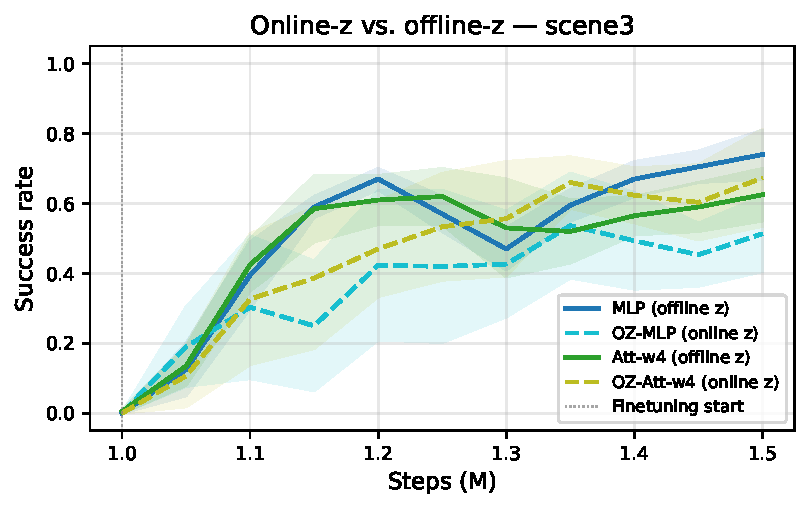
\includegraphics[width=\textwidth]{fig4_onlinez_comparison.pdf}
\caption{Fine-tuning learning curves on Scene3 for online-$z$ (dashed)
vs.\ offline-$z$ (solid) variants. Shaded bands: $\pm$1 std over 3 seeds.
Online-$z$ with attention (\textsc{OZ-Att-w4}) converges faster and to
a higher peak than either MLP variant.}
\label{fig:curves}
\end{figure}

Figure~\ref{fig:curves} shows that \textsc{OZ-Att-w4} converges faster and
to a higher peak than both offline variants.
The large seed variance in \textsc{OZ-Att-w4} ($0.50$--$0.88$) and
\textsc{OZ-MLP} ($0.46$--$0.74$) reveals sensitivity to the initial
quality of online-$z$ estimates early in fine-tuning.

\subsection{Window-Size Ablation}

\begin{figure}[t]
\centering
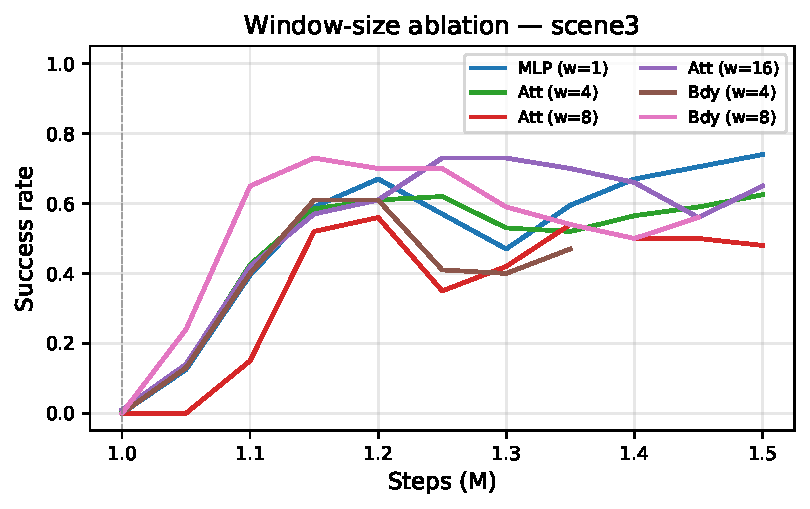
\includegraphics[width=\textwidth]{fig3_window_ablation.pdf}
\caption{Scene3 finetuning learning curves for offline-$z$ attention variants
at window sizes $K \in \{4,8,16\}$ compared to \textsc{MLP}.
Performance is non-monotone in $K$, motivating online-$z$.}
\label{fig:window_ablation}
\end{figure}

Performance is non-monotone in $K$ (Fig.~\ref{fig:window_ablation}).
Window 16 performs best (0.76), matching the MLP baseline;
window 8 performs worst (0.40).
We attribute this to variance in encoder initialization at intermediate
window sizes, where the encoder has enough context to overfit to
spurious temporal correlations but not enough to learn stable phase boundaries.

\subsection{Boundary-Aware Attention}

\begin{table}[t]
\centering
\caption{Standard vs.\ boundary-aware attention on Scene3 (offline $z$, seed 0).}
\label{tab:boundary}
\begin{tabular}{lcc}
\toprule
              & $w=4$ & $w=8$ \\
\midrule
Standard      & 0.68  & 0.40  \\
Boundary-aware & 0.42  & 0.66  \\
\bottomrule
\end{tabular}
\end{table}

Table~\ref{tab:boundary} shows a striking reversal: boundary masking
hurts at $w=4$ ($-0.26$) but helps at $w=8$ ($+0.26$).
At $w=4$, phase boundaries are rare within a short window and masking
zeros out valid tokens.
At $w=8$, windows regularly span sub-goal transitions; masking
cross-phase tokens prevents averaging conflicting intentions.

\subsection{Latent Intention Structure}

\begin{figure}[t]
\centering
\IfFileExists{tsne_intentions.pdf}{%
  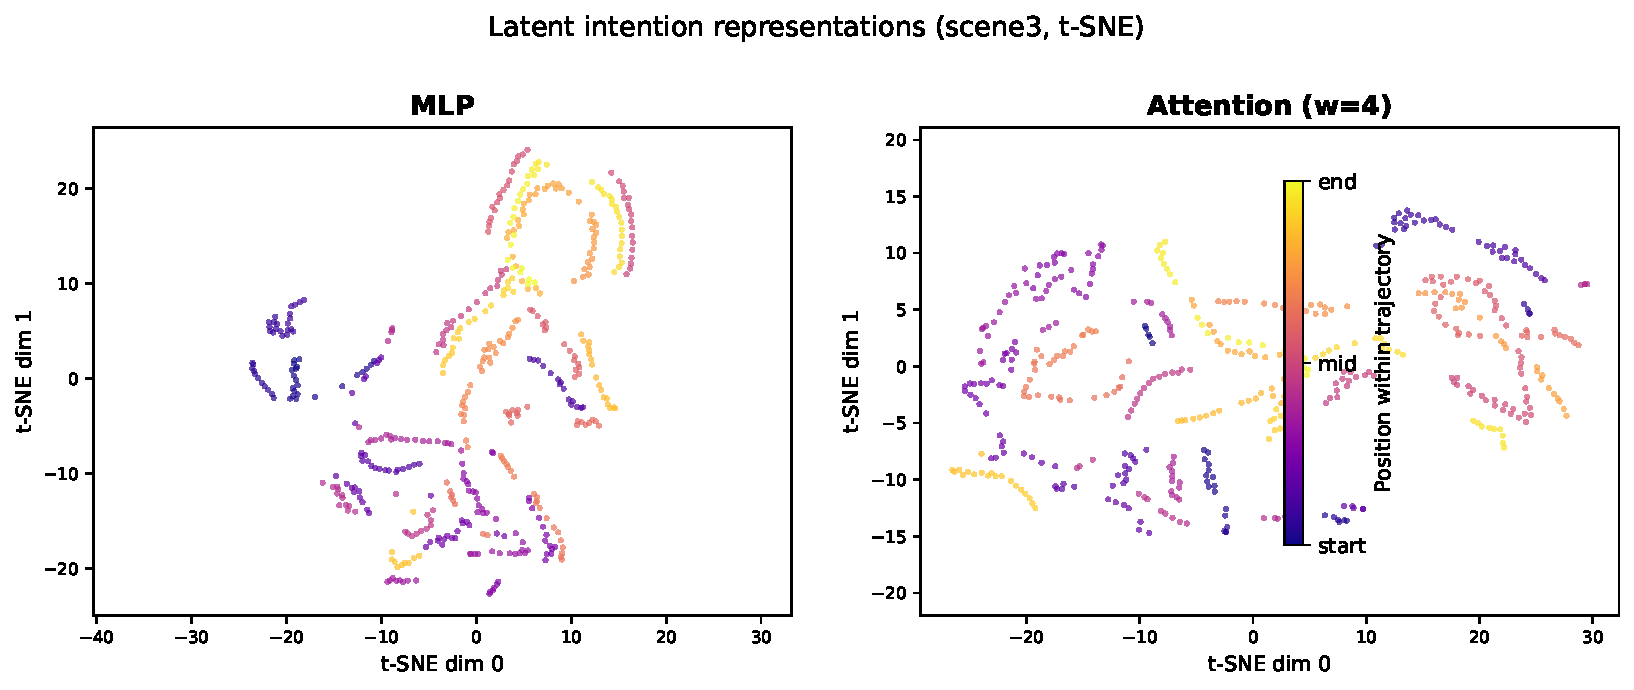
\includegraphics[width=\textwidth]{tsne_intentions.pdf}
}{%
  \fbox{\parbox{\textwidth}{\centering\vspace{1.5cm}
  t-SNE figure pending (job submitted, rendering now)
  \vspace{1.5cm}}}
}
\caption{t-SNE~\citep{maaten2008tsne} of latent intentions $z$ from 4000
Scene3 transitions, colored by normalized trajectory position
(purple = start, yellow = end).
Left: \textsc{MLP} encoder. Right: \textsc{Att-w4} encoder.
Structured clusters aligned with behavioral phases indicate that
the attention encoder better captures temporal context.}
\label{fig:tsne}
\end{figure}

Figure~\ref{fig:tsne} visualizes the latent space via
t-SNE~\citep{maaten2008tsne}.
An ideal intention encoder produces clusters corresponding to distinct
behavioral phases rather than tracking raw time.
The attention encoder's clusters should better align with semantic phases,
providing direct evidence that the multi-step window aids behavioral disambiguation.

\subsection{Visual Observations}

We integrated an IMPALA CNN encoder and submitted four jobs
(MLP, Att-w4/8/16) on the \textsc{visual-cube} environment.
Pixel-based pretraining is significantly slower ($\sim$10$\times$)
than state-based, and results were not available at submission time
due to compute constraints.
The engineering contributions (lazy normalization, flow-goal clipping
fix, window channel consistency) are described in Section~\ref{sec:visual}
and represent the necessary groundwork for future visual experiments.

% ============================================================
\section{Related Work}
\label{sec:related}
% ============================================================

\paragraph{Offline goal-conditioned RL.}
A large body of work learns goal-reaching from offline
data~\citep{ghosh2021gcsl,park2023hiql,eysenbach2022contrastive,park2025ogbenchbenchmarkingofflinegoalconditioned}.
IQL~\citep{kostrikov2021iql} provides the advantage-weighted BC used in fine-tuning.
Our work extends \base{}~\citep{zheng2025infom} and builds on
learning from passive data via latent intentions~\citep{ghosh2023passive}.

\paragraph{Successor representations and occupancy models.}
Successor representations~\citep{dayan1993successor,barreto2017sf}
underlie many goal-conditioned methods.
Flow-matching occupancy
models~\citep{farebrother2025tdflows,park2025flowq,dong2025valueflows}
directly parameterize the occupancy density.
The most closely related is TD flows~\citep{farebrother2025tdflows},
which also uses flow matching but relies on forward-backward
representations~\citep{touati2021fb} for intentions rather than learned latents.

\paragraph{Temporal context and sequence modeling.}
Decision Transformer~\citep{chen2021dt} and GATO~\citep{reed2022gato}
model full trajectories autoregressively.
Online DT~\citep{zheng2022odt} adds online fine-tuning, analogous to
our online-$z$.
Context-based meta-RL methods PEARL~\citep{rakelly2019pearl} and
RL$^2$~\citep{duan2016rl2} encode recent transitions as a context
vector for fast adaptation---our attention encoder and online-$z$ share
this spirit but operate in the offline-pretrain then online-deploy setting.

\paragraph{Mixture latent models.}
MoG posteriors appear in multi-modal imitation
learning~\citep{hausman2017multimodal} and InfoGAIL~\citep{li2017infogail}.
Boundary-aware attention shares spirit with hierarchical
attention~\citep{yang2016hierarchical} and segment-aware transformers.

\paragraph{Visual RL.}
IMPALA~\citep{espeholt2018impala} and CURL~\citep{laskin2020curl}
are standard pixel encoders for RL.
Our visual extension brings \base{} toward image-based manipulation settings.

\paragraph{RL with flow-matching.}
Diffuser~\citep{janner2022diffuser} and Diffusion
Policy~\citep{chi2023diffusionpolicy} model trajectories with diffusion.
Flow Q-learning~\citep{park2025flowq} and Value
Flows~\citep{dong2025valueflows} apply flow matching to Q-functions.

% ============================================================
\section{Discussion and Conclusion}
\label{sec:conclusion}
% ============================================================

We presented five extensions to \base{}~\citep{zheng2025infom}:
a MoG encoder, an attention encoder, boundary-aware attention,
online-$z$ conditioning, and pixel observation support.

Our central finding is that \emph{temporal context in intention inference
is beneficial only when inference is performed online at deployment time}.
Offline attention underperforms the MLP baseline; online attention
yields a peak $+22\%$ absolute gain on Scene3.
This reveals a fundamental tension in offline RL:
intention labels inferred from a fixed dataset reflect a labeling
policy, not the policy being learned---any mismatch degrades test-time performance.

The MoG encoder provides marginal gains on Scene3 and hurts on Cube2/Puzzle,
suggesting multi-modality in the posterior is less critical than temporal context.
Boundary-aware attention shows the clearest theoretical motivation
but mixed results: it helps at $w=8$ (where phase transitions are common)
and hurts at $w=4$.
A learned boundary detector may be more robust than the heuristic used here.

\paragraph{Limitations.}
Visual (pixel-based) results are pending due to compute constraints.
All experiments are single-codebase; hyperparameter sensitivity is not
fully characterized.
Seed variance in online-$z$ variants is high, suggesting the method
would benefit from more stable initialization of the rolling buffer.

\paragraph{Future work.}
Natural extensions: (1) hierarchical online-$z$ inferring both sub-goal
and style; (2) meta-learning the encoder across diverse tasks for
out-of-distribution generalization~\citep{rakelly2019pearl};
(3) replacing the heuristic boundary detector with a learned one.

\clearpage

\acknowledgments{Experiments were run on the Princeton Della GPU cluster.
The base \base{} codebase was released by \citet{zheng2025infom} under
an open-source license; this work builds directly on it.}

\bibliography{references}

\end{document}
